\documentclass[12pt]{article}            % Report class in 11 points
\parindent0pt  \parskip12pt             % make block paragraphs
\usepackage{graphicx}
\usepackage{listings}
\graphicspath{ {images/} }
\usepackage{graphicx} %  graphics header file
\begin{document}
\begin{titlepage}
    \centering
  \vfill
    
\includegraphics[width=8cm]{uni_logo.png} \\ 
	\vskip2cm
    {\bfseries\Large
	Data Structures and Algorithms \\ (CS09203)\\
	
	\vskip2cm
	Lab Report 
	 
	\vskip2cm
	}    

\begin{center}
\begin{tabular}{ l l  } 

Name: & Rehman ullah baig \\ 
Registration \#: &CSU-F16118 \\ 
Lab Report \#: & 10 \\ 
 Dated:& 18-06-2018\\ 
Submitted To:& Mr. Usman Ahmed\\ 

 %\hline
\end{tabular}
\end{center}
    \vfill
    The University of Lahore, Islamabad Campus\\
Department of Computer Science \& Information Technology
\end{titlepage}


    
    {\bfseries\Large
\centering
	Experiment \#10 \\

The Breadth-first search algorithm\\
	
	}    
 \vskip1cm
 \textbf {Objective}\\  To understand and implement The Breath-first search algorithm.
 
 \textbf {Software Tool} \\
1. Windows 7  \\
2. Dev C++\\
3. Miktex   \\

\section{Theory }              
A standard BFS implementation puts each vertex of the graph into one of two categories:

Visited
Not Visited
The purpose of the algorithm is to mark each vertex as visited while avoiding cycles.

The algorithm works as follows: \\
The BFS algorithm works as follows:\\
1.	Start by putting any one of the graph's vertices on top of a Queue.\\
2.	Take the top item of the stack and add it to the visited list.\\
3.	Create a list of that vertex's adjacent nodes. Add the ones which aren't in the visited list to the top of Queue. \\
4.	Keep repeating steps 2 and 3 until the stack is empty.\\ \\

\section{Task}  
\subsection{Procedure: Task 1 }     

\begin{figure*}
\centering
  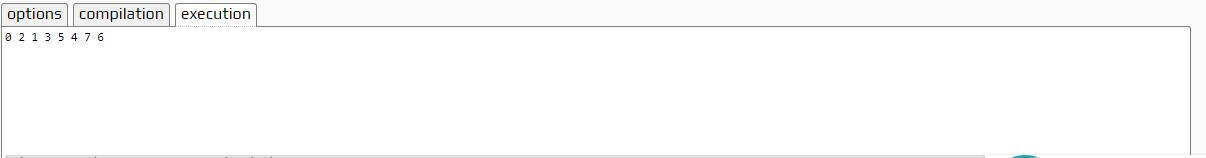
\includegraphics[width=12cm,height=6cm,keepaspectratio]{3.png}
\caption{Data entering into different locations}
\label{Figure:3}    
\end{figure*}
Note that the above code traverses only the vertices reachable from a given source vertex. All the vertices may not be reachable from a given vertex (example Disconnected graph). To print all the vertices, we can modify the BFS function to do traversal starting from all nodes one by one (Like the DFS modified version) .

Time Complexity: O(V+E) where V is number of vertices in the graph and E is number of edges in the graph.

\subsection{Procedure: Task 2 }     

\begin{lstlisting}[language=C++]



#include<iostream>
#include<queue>
using namespace std;

struct Node {
	char data;
	Node *left;
	Node *right;
};

void LevelOrder(Node *root) {
	if(root == NULL) return;
	queue<Node*> Q;
	Q.push(root);  

	while(!Q.empty()) {
		Node* current = Q.front();
		Q.pop(); 
		cout<<current->data<<" ";
		if(current->left != NULL) Q.push(current->left);
		if(current->right != NULL) Q.push(current->right);
	}
}
Node* Insert(Node *root,char data) {
	if(root == NULL) {
		root = new Node();
		root->data = data;
		root->left = root->right = NULL;
	}
	else if(data <= root->data) root->left = Insert(root->left,data);
	else root->right = Insert(root->right,data);
	return root;
}

int main() {

	Node* root = NULL;
	root = Insert(root,'0'); root = Insert(root,'2');
	root = Insert(root,'1'); root = Insert(root,'3'); 
	root = Insert(root,'5'); root = Insert(root,'7');
          root = Insert(root,'6'); root = Insert(root,'4');
	LevelOrder(root);
}
\end{lstlisting}

\section{Conclusion}  
Breadth-First search is like traversing a tree where each node is a state which may a be a potential candidate for solution. It expands nodes from the root of the tree and then generates one level of the tree at a time until a solution is found. It is very easily implemented by maintaining a queue of nodes. 
 
\end{document}                          % The required last line
